\Chapter{Magic}
{The Tablelands are a giant wasteland, to the untrained eye barren and devoid of life. When people see plants wither and die when someone utters mysterious phrases accompanied by unknown gestures, they assume the worst. They cry wizard and the mob instantly gathers to kill him. But if people venture into the wastes and look under the rocks, they will learn that Athas is teeming with all sorts of life. And when the vermin swarm forth to envelop them, biting and crawling into every orifice, do they see the irony?}
{The Oracle, Blue Shrine Scrolls}

\Capitalize{T}{he} abuse of magic has shaped and scarred the world of Athas in the past 8,000 years. Because of that magic is universally feared and hated by the general populace. Wizards are outlaws that are hunted and killed by templars. Magic is hard to find, and even low-level spells are not easily accessible.

A spell is a one-time magical effect. Spells come in two types: arcane (cast by wizards) and divine (cast by clerics, druids, experienced rangers, and templars). Some spellcasters select their spells from a limited list of spells known, while others have access to a wide variety of options.

Most spellcasters prepare their spells in advance---whether from a spellbook or through devout prayers and meditation---while some cast spells spontaneously without preparation.

Despite these different ways that characters use to learn or prepare their spells, when it comes to casting them, the spells are very much alike.

Cutting across the categories of arcane and divine spells are the eight schools of magic. These schools represent the different ways that spells take effect.

\begin{figure*}[t!]
\centering
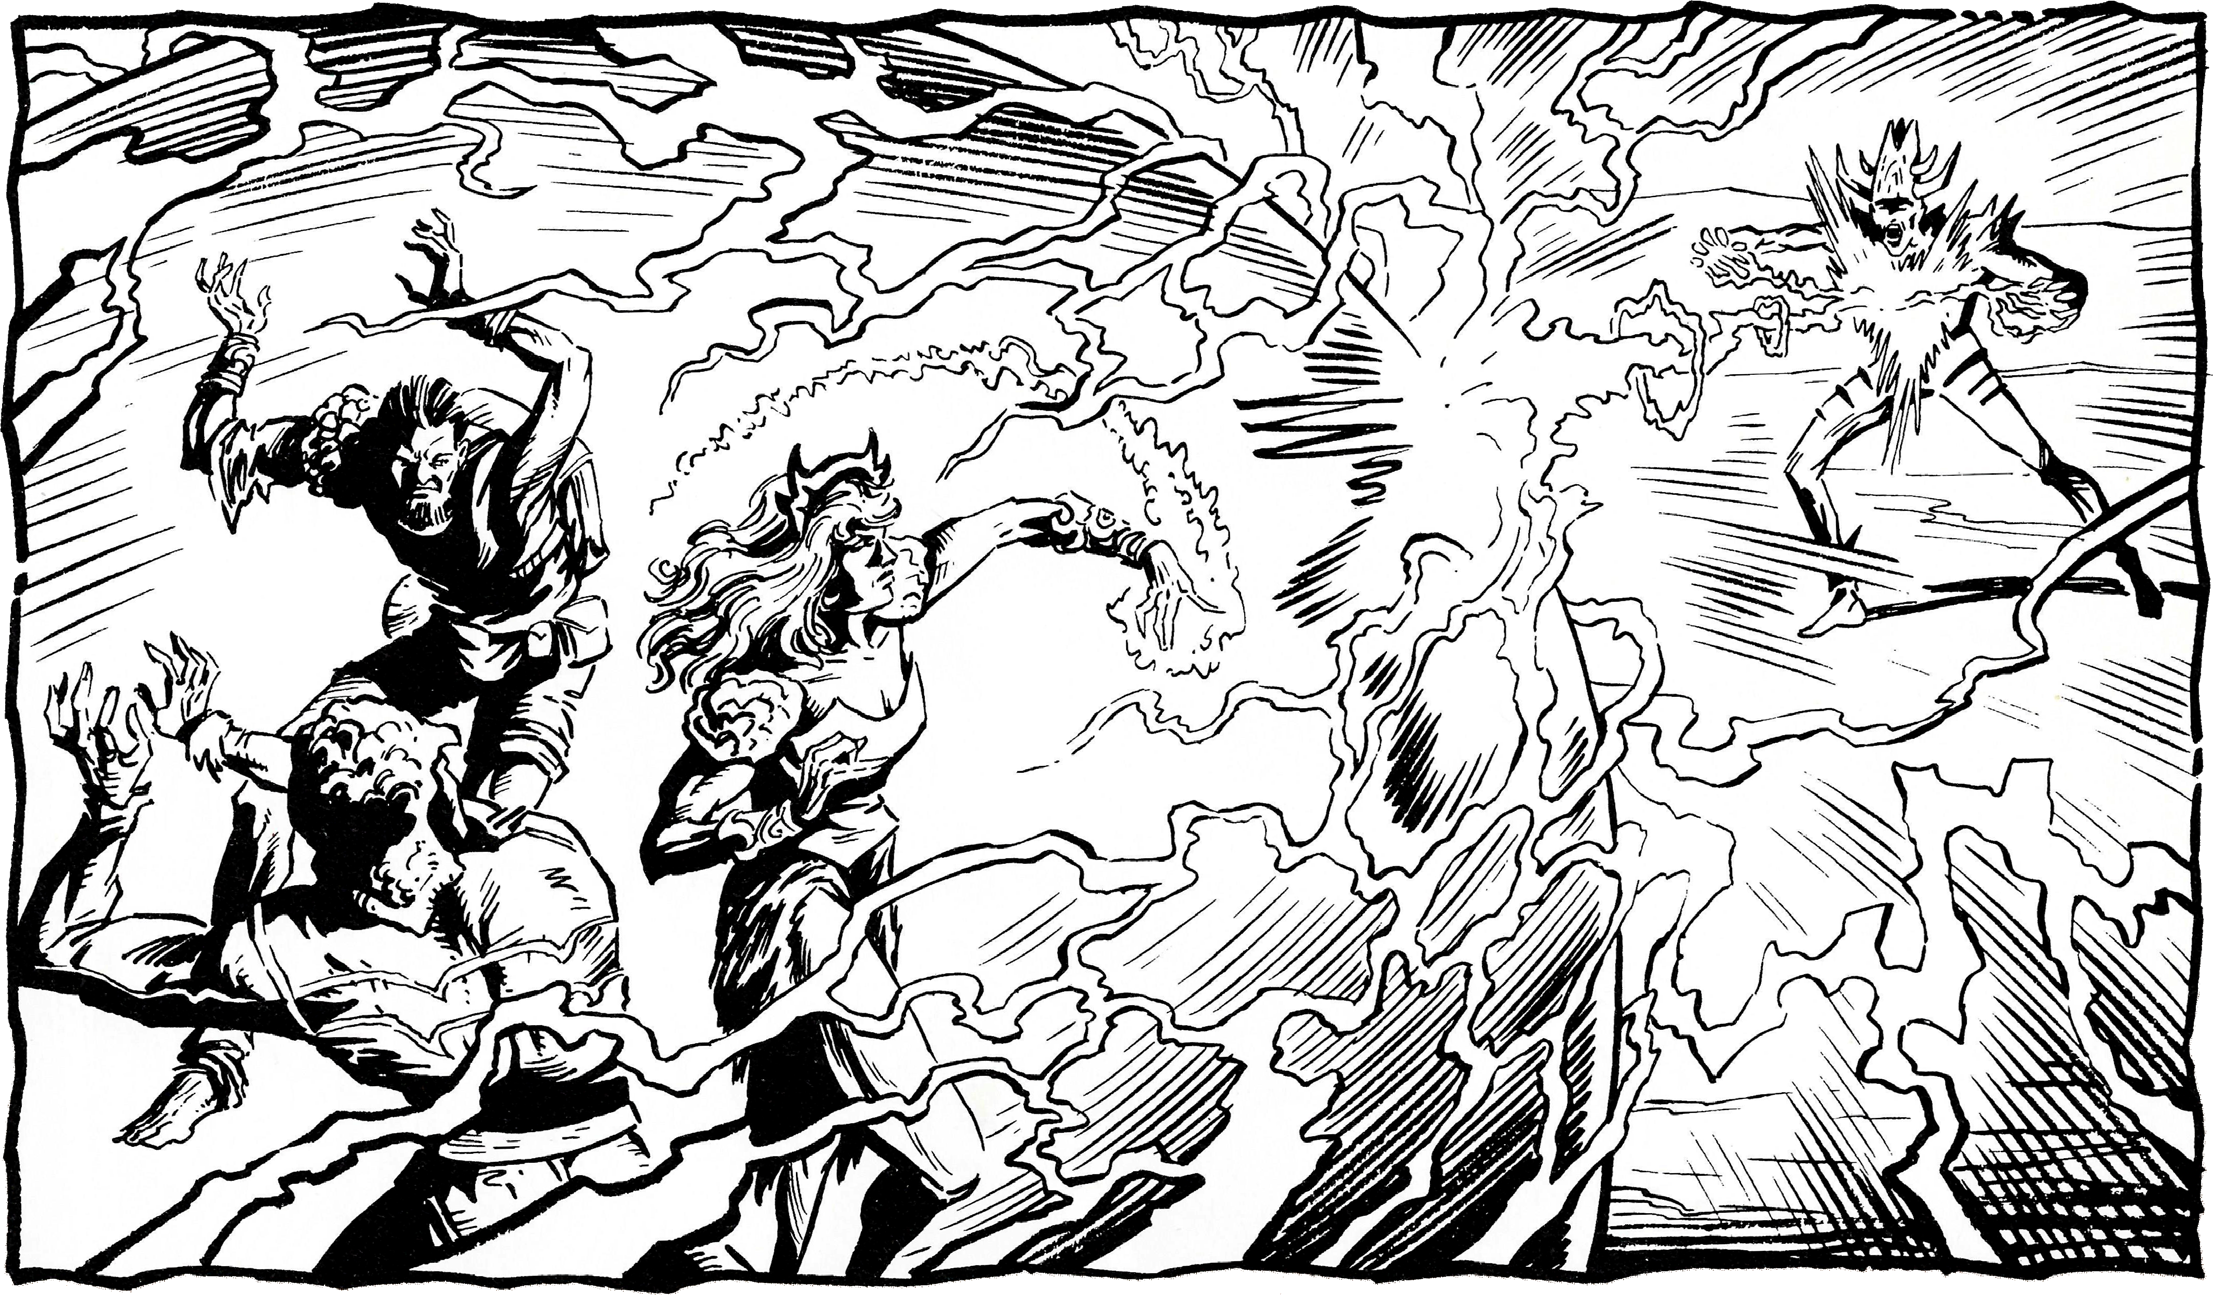
\includegraphics[width=\textwidth]{images/magic-1.png}
\WOTC
\end{figure*}

\Figure*{t}{images/magic-1.png}
\section{Casting Spells}
Whether a spell is arcane or divine, and whether a character prepares spells in advance or chooses them on the spot, casting a spell works the same way.

\subsection{Choosing A Spell}
First you must choose which spell to cast. If you're a cleric, druid, experienced ranger, or wizard, you select from among spells prepared earlier in the day and not yet cast (see Preparing Wizard Spells and Preparing Divine Spells).

If you're a templar, you can select any spell you know, provided you are capable of casting spells of that level or higher.

To cast a spell, you must be able to speak (if the spell has a verbal component), gesture (if it has a somatic component), and manipulate the material components or focus (if any). Additionally, you must concentrate to cast a spell.

If a spell has multiple versions, you choose which version to use when you cast it. You don't have to prepare a specific version of the spell.

Once you've cast a prepared spell, you can't cast it again until you prepare it again. (If you've prepared multiple copies of a single spell, you can cast each copy once.) If you're a templar, casting a spell counts against your daily limit for spells of that spell level, but you can cast the same spell again if you haven't reached your limit.

\subsection{Concentration}
To cast a spell, you must concentrate. If something interrupts your concentration while you're casting, you must make a \skill{Concentration} check or lose the spell. The more distracting the interruption and the higher the level of the spell you are trying to cast, the higher the DC is. If you fail the check, you lose the spell just as if you had cast it to no effect.

\textbf{Injury}: If while trying to cast a spell you take damage, you must make a \skill{Concentration} check (DC 10 + points of damage taken + the level of the spell you're casting). If you fail the check, you lose the spell without effect. The interrupting event strikes during spellcasting if it comes between when you start and when you complete a spell (for a spell with a casting time of 1 full round or more) or if it comes in response to your casting the spell (such as an attack of opportunity provoked by the spell or a contingent attack, such as a readied action).

If you are taking continuous damage half the damage is considered to take place while you are casting a spell. You must make a \skill{Concentration} check (DC 10 + \onehalf the damage that the continuous source last dealt + the level of the spell you're casting). If the last damage dealt was the last damage that the effect could deal then the damage is over, and it does not distract you.

Repeated damage does not count as continuous damage.

\textbf{Spell}: If you are affected by a spell while attempting to cast a spell of your own, you must make a \skill{Concentration} check or lose the spell you are casting. If the spell affecting you deals damage, the DC is 10 + points of damage + the level of the spell you're casting.

If the spell interferes with you or distracts you in some other way, the DC is the spell's saving throw DC + the level of the spell you're casting. For a spell with no saving throw, it's the DC that the spell's saving throw would have if a save were allowed.

\textbf{Grappling or Pinned}: The only spells you can cast while grappling or pinned are those without somatic components and whose material components (if any) you have in hand. Even so, you must make a \skill{Concentration} check (DC 20 + the level of the spell you're casting) or lose the spell.

\textbf{Vigorous Motion}: If you are riding on a moving mount, taking a bouncy ride in a wagon, on a small boat in rough water, below-decks in a storm-tossed ship, or simply being jostled in a similar fashion, you must make a \skill{Concentration} check (DC 10 + the level of the spell you're casting) or lose the spell.

\textbf{Violent Motion}: If you are on a galloping horse, taking a very rough ride in a wagon, on a small boat in rapids or in a storm, on deck in a storm-tossed ship, or being tossed roughly about in a similar fashion, you must make a \skill{Concentration} check (DC 15 + the level of the spell you're casting) or lose the spell.

\textbf{Violent Weather}: You must make a \skill{Concentration} check if you try to cast a spell in violent weather. If you are in a high wind carrying blinding rain or sleet, the DC is 5 + the level of the spell you're casting. If you are in wind-driven hail, dust, or debris, the DC is 10 + the level of the spell you're casting. In either case, you lose the spell if you fail the \skill{Concentration} check. If the weather is caused by a spell, use the rules in the Spell subsection above.

\textbf{Casting Defensively}: If you want to cast a spell without provoking any attacks of opportunity, you must make a \skill{Concentration} check (DC 15 + the level of the spell you're casting) to succeed. You lose the spell if you fail.

\textbf{Entangled}: If you want to cast a spell while entangled in a net or by a tanglefoot bag or while you're affected by a spell with similar effects, you must make a DC 15 \skill{Concentration} check to cast the spell. You lose the spell if you fail.
\subsection{Counterspells}
It is possible to cast any spell as a counterspell. By doing so, you are using the spell's energy to disrupt the casting of the same spell by another character. Counterspelling works even if one spell is divine and the other arcane.

\textbf{How Counterspells Work:} To use a counterspell, you must select an opponent as the target of the counterspell. You do this by choosing the ready action. In doing so, you elect to wait to complete your action until your opponent tries to cast a spell. (You may still move your speed, since ready is a standard action.)

If the target of your counterspell tries to cast a spell, make a \skill{Spellcraft} check (DC 15 + the spell's level). This check is a free action. If the check succeeds, you correctly identify the opponent's spell and can attempt to counter it. If the check fails, you can't do either of these things.

To complete the action, you must then cast the correct spell. As a general rule, a spell can only counter itself. If you are able to cast the same spell and you have it prepared (if you prepare spells), you cast it, altering it slightly to create a counterspell effect. If the target is within range, both spells automatically negate each other with no other results.

\textbf{Counterspelling Metamagic Spells:} Metamagic feats are not taken into account when determining whether a spell can be countered

\textbf{Specific Exceptions:} Some spells specifically counter each other, especially when they have diametrically opposed effects.

\textbf{Dispel Magic as a Counterspell:} You can use dispel magic to counterspell another spellcaster, and you don't need to identify the spell he or she is casting. However, dispel magic doesn't always work as a counterspell.

\subsection{Caster Level}
A spell's power often depends on its caster level, which for most spellcasting characters is equal to your class level in the class you're using to cast the spell.

You can cast a spell at a lower caster level than normal, but the caster level you choose must be high enough for you to cast the spell in question, and all level-dependent features must be based on the same caster level.

In the event that a class feature, domain granted power, or other special ability provides an adjustment to your caster level, that adjustment applies not only to effects based on caster level (such as range, duration, and damage dealt) but also to your caster level check to overcome your target's spell resistance and to the caster level used in dispel checks (both the dispel check and the DC of the check).

\textbf{Caster Level Checks:} To make a caster level check, roll 1d20 and add your caster level (in the relevant class). If the result equals or exceeds the DC (or the spell resistance, in the case of caster level checks made for spell resistance), the check succeeds.

\subsection{Spell Failure}
If you ever try to cast a spell in conditions where the characteristics of the spell cannot be made to conform, the casting fails and the spell is wasted.

Spells also fail if your concentration is broken and might fail if you're wearing armor while casting a spell with somatic components.

\subsection{The Spell's Result}
Once you know which creatures (or objects or areas) are affected, and whether those creatures have made successful saving throws (if any were allowed), you can apply whatever results a spell entails.

\Figure*{t}{images/magic-3.png}
\subsection{Special Spell Effects}
Many special spell effects are handled according to the school of the spells in question Certain other special spell features are found across spell schools.

\textbf{Attacks:} Some spell descriptions refer to attacking. All offensive combat actions, even those that don't damage opponents are considered attacks. Attempts to turn or rebuke undead count as attacks. All spells that opponents resist with saving throws, that deal damage, or that otherwise harm or hamper subjects are attacks. Spells that summon monsters or other allies are not attacks because the spells themselves don't harm anyone.

\textbf{Bonus Types:} Usually, a bonus has a type that indicates how the spell grants the bonus. The important aspect of bonus types is that two bonuses of the same type don't generally stack. With the exception of dodge bonuses, most circumstance bonuses, and racial bonuses, only the better bonus works (see Combining Magical Effects, below). The same principle applies to penalties---a character taking two or more penalties of the same type applies only the worst one.

\textbf{Bringing Back the Dead:} Several spells have the power to restore slain characters to life.

When a living creature dies, its soul departs its body, leaves the Material Plane, travels through the Astral Plane, and goes to abide on the plane where the creature's deity resides. If the creature did not worship a deity, its soul departs to the plane corresponding to its alignment. Bringing someone back from the dead means retrieving his or her soul and returning it to his or her body.

\textit{Level Loss:} Any creature brought back to life usually loses one level of experience. The character's new XP total is midway between the minimum needed for his or her new (reduced) level and the minimum needed for the next one. If the character was 1st level at the time of death, he or she loses 2 points of Constitution instead of losing a level.

This level loss or Constitution loss cannot be repaired by any mortal means, even \spell{wish} or \spell{miracle}. A revived character can regain a lost level by earning XP through further adventuring. A revived character who was 1st level at the time of death can regain lost points of Constitution by improving his or her Constitution score when he or she attains a level that allows an ability score increase.

\textit{Preventing Revivification:} Enemies can take steps to make it more difficult for a character to be returned from the dead. Keeping the body prevents others from using \spell{raise dead} or \spell{resurrection} to restore the slain character to life. Casting \spell{trap the soul} prevents any sort of revivification unless the soul is first released.

\textit{Revivification against One's Will:} A soul cannot be returned to life if it does not wish to be. A soul knows the name, alignment, and patron deity (if any) of the character attempting to revive it and may refuse to return on that basis.


\subsection{Combining Magical Effects}
Spells or magical effects usually work as described, no matter how many other spells or magical effects happen to be operating in the same area or on the same recipient. Except in special cases, a spell does not affect the way another spell operates. Whenever a spell has a specific effect on other spells, the spell description explains that effect. Several other general rules apply when spells or magical effects operate in the same place:

\textbf{Stacking Effects:} Spells that provide bonuses or penalties on attack rolls, damage rolls, saving throws, and other attributes usually do not stack with themselves. More generally, two bonuses of the same type don't stack even if they come from different spells (or from effects other than spells; see Bonus Types, above).

\textit{Different Bonus Names:} The bonuses or penalties from two different spells stack if the modifiers are of different types. A bonus that isn't named stacks with any bonus.

\textit{Same Effect More than Once in Different Strengths:} In cases when two or more identical spells are operating in the same area or on the same target, but at different strengths, only the best one applies.

\textit{Same Effect with Differing Results:} The same spell can sometimes produce varying effects if applied to the same recipient more than once. Usually the last spell in the series trumps the others. None of the previous spells are actually removed or dispelled, but their effects become irrelevant while the final spell in the series lasts.

\textit{One Effect Makes Another Irrelevant:} Sometimes, one spell can render a later spell irrelevant. Both spells are still active, but one has rendered the other useless in some fashion.

\textit{Multiple Mental Control Effects:} Sometimes magical effects that establish mental control render each other irrelevant, such as a spell that removes the subjects ability to act. Mental controls that don't remove the recipient's ability to act usually do not interfere with each other. If a creature is under the mental control of two or more creatures, it tends to obey each to the best of its ability, and to the extent of the control each effect allows. If the controlled creature receives conflicting orders simultaneously, the competing controllers must make opposed Charisma checks to determine which one the creature obeys.

\textbf{Spells with Opposite Effects:} Spells with opposite effects apply normally, with all bonuses, penalties, or changes accruing in the order that they apply. Some spells negate or counter each other. This is a special effect that is noted in a spell's description.

\textbf{Instantaneous Effects:} Two or more spells with instantaneous durations work cumulatively when they affect the same target.
\subsection{Sensory Effects}
The stealthy preserver crouches low behind the stone walls of the ruins, fumbling through his belt pouch for his material components, peering cautiously around for signs of the approaching gith marauders. Breathless, he draws out his precious may also have effects that appeal to the senses of components and begins his chant and hand motions. Verbal, somatic, and material components are all in play, but what's really happening? What are the sensory effects associated with casting a spell?

On Athas the casting of magical spells often draws unwanted attention. The sensory effects of casting and the ways a wizard might cover, expand, or mimic them are acutely important. These sensory effects relate directly to detection; the greater the effects during casting, the greater the chance the wizard is found out. Of course, when a wizard wishes to dramatically announce his spellcasting abilities, the greater the effects the better.

All spells have both a visual and aural effect during casting. Middle-level (4th- to 6th-level) spells may also have effects that appeal to the senses of touch and smell. High-level spells may have grand effects.

Sensory effects for casting are particular to each spellcaster. The effects themselves remain constant for each sensory category, no matter what the spell level.

\textbf{Visual effects:} Streaks of sparkling multicolored light emerge from the vanishing material components, follow the movements of the spell's somatics (if any), then settle on the subject of the spell. The sparkling lights slightly illuminate the caster and target of the spell for the spell's entire casting time. Brightness is determined by spell level; color varies by spell and by caster. Other possible effects include glowing rings of light, heatless flames, and so on. A visual effect cannot substitute for an existing spell such as \spell{light} or the various illusions.

\textbf{Aural effects:} Along with any verbal components, a shimmer like that of tiny, metal wind chimes accompanies the caster's words, rising and falling with the spell's somatics. The jingling emanates from the caster's location, rising from silence to its maximum volume and back to silence over the casting time. Volume is determined by spell level. Other possible effects include a roaring wind, thousands of slithering snakes, etc.

\textbf{Olfactory effects:} For spells with olfactory sensory effects, an odor unique to the caster or the spell permeates the air. The smell may be pleasant, such as flowers or perfumes, or quite unpleasant, such as rotting meat. Intensity of the smell is determined by spell level.

\textbf{Tactile effects:} Creatures near the caster feel something brush up against them. The nature of the sensation can be soft and pleasant, such as feathers, or abrasive, such as grit or jagged bone. Intensity of the sensation is determined by spell level.

\textbf{Grand effects:} Spells of especially high level may cause grand effects in casting. The ground may tremble, rocking tables and tipping over bottles. The weather may temporarily change, clouding over ominously, wind picking up or stopping, temperature growing abnormally hot or chill.

\Table{Sensory Effects of Casting}{lCCC}{
\tableheader Spell Level & \tableheader Visual/Aural & \tableheader Olfactory/Tacticle & \tableheader Grand \\
1st--3rd & Yes & No       & No       \\
4th--6th & Yes & Optional & No       \\
7th--9th & Yes & Yes      & Optional \\
}


\subsubsection{Detecting Spellcasting}
Whenever a spell is cast, there is a chance that any casual observer will notice it. Aural and visual effects require \skill{Listen} and \skill{Spot} checks, respectively. Olfactory and tacticle effects require Wisdom checks, and the DC increases by 1 for each 3 meters of distance between the spellcaster and the observer. Grand effects are automatically detected. DC for each check is 10 minus the spell level.

% \Table{Sensory Range}{lCCC}{
% \tableheader Spell Level & \tableheader Visual/Aural & \tableheader Olfactory/Tacticle & \tableheader Grand \\
% 1st--3rd & 18 m &      &      \\
% 4th--6th & 27 m & 18 m &      \\
% 7th--9th & 36 m & 27 m & 36 m \\	
% }


\section{Spell Descriptions}
The description of each spell is presented in a standard format. Each category of information is explained and defined below.


\subsection{Name}
The first line of every spell description gives the name by which the spell is generally known.

\subsection{School (Subschool)}
Beneath the spell name is a line giving the school of magic (and the subschool, if appropriate) that the spell belongs to.

Almost every spell belongs to one of eight schools of magic. A school of magic is a group of related spells that work in similar ways. A small number of spells (arcane mark, limited wish, permanency, prestidigitation, and wish) are universal, belonging to no school.

\textbf{Abjuration}: Abjurations are protective spells. They create physical or magical barriers, negate magical or physical abilities, harm trespassers, or even banish the subject of the spell to another plane of existence.

If one abjuration spell is active within 10 feet of another for 24 hours or more, the magical fields interfere with each other and create barely visible energy fluctuations. The DC to find such spells with the Search skill drops by 4.

If an abjuration creates a barrier that keeps certain types of creatures at bay, that barrier cannot be used to push away those creatures. If you force the barrier against such a creature, you feel a discernible pressure against the barrier. If you continue to apply pressure, you end the spell.

\textbf{Conjuration}: Each conjuration spell belongs to one of five subschools. Conjurations bring manifestations of objects, creatures, or some form of energy to you (the summoning subschool), actually transport creatures from another plane of existence to your plane (calling), heal (healing), transport creatures or objects over great distances (teleportation), or create objects or effects on the spot (creation). Creatures you conjure usually, but not always, obey your commands.

A creature or object brought into being or transported to your location by a conjuration spell cannot appear inside another creature or object, nor can it appear floating in an empty space. It must arrive in an open location on a surface capable of supporting it.

The creature or object must appear within the spell's range, but it does not have to remain within the range.

\textit{Calling}: A calling spell transports a creature from another plane to the plane you are on. The spell grants the creature the one-time ability to return to its plane of origin, although the spell may limit the circumstances under which this is possible. Creatures who are called actually die when they are killed; they do not disappear and reform, as do those brought by a summoning spell (see below). The duration of a calling spell is instantaneous, which means that the called creature can't be dispelled.

\textit{Creation}: A creation spell manipulates matter to create an object or creature in the place the spellcaster designates (subject to the limits noted above). If the spell has a duration other than instantaneous, magic holds the creation together, and when the spell ends, the conjured creature or object vanishes without a trace. If the spell has an instantaneous duration, the created object or creature is merely assembled through magic. It lasts indefinitely and does not depend on magic for its existence.

\textit{Healing}: Certain divine conjurations heal creatures or even bring them back to life.

\textit{Summoning}: A summoning spell instantly brings a creature or object to a place you designate. When the spell ends or is dispelled, a summoned creature is instantly sent back to where it came from, but a summoned object is not sent back unless the spell description specifically indicates this. A summoned creature also goes away if it is killed or if its hit points drop to 0 or lower. It is not really dead. It takes 24 hours for the creature to reform, during which time it can't be summoned again.

When the spell that summoned a creature ends and the creature disappears, all the spells it has cast expire. A summoned creature cannot use any innate summoning abilities it may have, and it refuses to cast any spells that would cost it XP, or to use any spell-like abilities that would cost XP if they were spells.

\textit{Teleportation}: A teleportation spell transports one or more creatures or objects a great distance. The most powerful of these spells can cross planar boundaries. Unlike summoning spells, the transportation is (unless otherwise noted) one-way and not dispellable.

Teleportation is instantaneous travel through the Astral Plane. Anything that blocks astral travel also blocks teleportation.

\textbf{Divination}: Divination spells enable you to learn secrets long forgotten, to predict the future, to find hidden things, and to foil deceptive spells.

Many divination spells have cone-shaped areas. These move with you and extend in the direction you look. The cone defines the area that you can sweep each round. If you study the same area for multiple rounds, you can often gain additional information, as noted in the descriptive text for the spell.

\textit{Scrying}: A scrying spell creates an invisible magical sensor that sends you information. Unless noted otherwise, the sensor has the same powers of sensory acuity that you possess. This level of acuity includes any spells or effects that target you, but not spells or effects that emanate from you. However, the sensor is treated as a separate, independent sensory organ of yours, and thus it functions normally even if you have been blinded, deafened, or otherwise suffered sensory impairment.

Any creature with an Intelligence score of 12 or higher can notice the sensor by making a DC 20 Intelligence check. The sensor can be dispelled as if it were an active spell.

Lead sheeting or magical protection blocks a scrying spell, and you sense that the spell is so blocked.

\textbf{Enchantment}: Enchantment spells affect the minds of others, influencing or controlling their behavior.

All enchantments are mind-affecting spells. Two types of enchantment spells grant you influence over a subject creature.

\textit{Charm}: A charm spell changes how the subject views you, typically making it see you as a good friend.

\textit{Compulsion}: A compulsion spell forces the subject to act in some manner or changes the way her mind works. Some compulsion spells determine the subject's actions or the effects on the subject, some compulsion spells allow you to determine the subject's actions when you cast the spell, and others give you ongoing control over the subject.

\textbf{Evocation}: Evocation spells manipulate energy or tap an unseen source of power to produce a desired end. In effect, they create something out of nothing. Many of these spells produce spectacular effects, and evocation spells can deal large amounts of damage.

\textbf{Illusion}: Illusion spells deceive the senses or minds of others. They cause people to see things that are not there, not see things that are there, hear phantom noises, or remember things that never happened.

\textit{Figment}: A figment spell creates a false sensation. Those who perceive the figment perceive the same thing, not their own slightly different versions of the figment. (It is not a personalized mental impression.) Figments cannot make something seem to be something else. A figment that includes audible effects cannot duplicate intelligible speech unless the spell description specifically says it can. If intelligible speech is possible, it must be in a language you can speak. If you try to duplicate a language you cannot speak, the image produces gibberish. Likewise, you cannot make a visual copy of something unless you know what it looks like.

Because figments and glamers (see below) are unreal, they cannot produce real effects the way that other types of illusions can. They cannot cause damage to objects or creatures, support weight, provide nutrition, or provide protection from the elements. Consequently, these spells are useful for confounding or delaying foes, but useless for attacking them directly.

A figment's AC is equal to 10 + its size modifier.

\textit{Glamer}: A glamer spell changes a subject's sensory qualities, making it look, feel, taste, smell, or sound like something else, or even seem to disappear.

\textit{Pattern}: Like a figment, a pattern spell creates an image that others can see, but a pattern also affects the minds of those who see it or are caught in it. All patterns are mind-affecting spells.

\textit{Phantasm}: A phantasm spell creates a mental image that usually only the caster and the subject (or subjects) of the spell can perceive. This impression is totally in the minds of the subjects. It is a personalized mental impression. (It's all in their heads and not a fake picture or something that they actually see.) Third parties viewing or studying the scene don't notice the phantasm. All phantasms are mind-affecting spells.

\textit{Shadow}: A shadow spell creates something that is partially real from extradimensional energy. Such illusions can have real effects. Damage dealt by a shadow illusion is real.

\textit{Saving Throws and Illusions (Disbelief)}: Creatures encountering an illusion usually do not receive saving throws to recognize it as illusory until they study it carefully or interact with it in some fashion.

A successful saving throw against an illusion reveals it to be false, but a figment or phantasm remains as a translucent outline.

A failed saving throw indicates that a character fails to notice something is amiss. A character faced with proof that an illusion isn't real needs no saving throw. If any viewer successfully disbelieves an illusion and communicates this fact to others, each such viewer gains a saving throw with a +4 bonus.

\textbf{Necromancy}: Necromancy spells manipulate the power of death, unlife, and the life force. Spells involving undead creatures make up a large part of this school.

\textbf{Transmutation}: Transmutation spells change the properties of some creature, thing, or condition.


\subsection{[Descriptor]}
Appearing on the same line as the school and subschool, when applicable, is a descriptor that further categorizes the spell in some way. Some spells have more than one descriptor.

The descriptors are acid, air, chaotic, cold, darkness, death, earth, electricity, evil, fear, fire, force, good, language-dependent, lawful, light, mind-affecting, ritual, sonic, and water.

Most of these descriptors have no game effect by themselves, but they govern how the spell interacts with other spells, with special abilities, with unusual creatures, with alignment, and so on.

A language-dependent spell uses intelligible language as a medium for communication. If the target cannot understand or cannot hear what the caster of a language-dependent spell says the spell fails.

A mind-affecting spell works only against creatures with an Intelligence score of 1 or higher.

A ritual spell can be cast following the normal rules for spellcasting, or the spell can be cast as a ritual.


\subsection{Level}
The next line of a spell description gives the spell's level, a number between 0 and 9 that defines the spell's relative power. This number is preceded by an abbreviation for the class whose members can cast the spell. The Level entry also indicates whether a spell is a domain spell and, if so, what its domain and its level as a domain spell are. A spell's level affects the DC for any save allowed against the effect.

Names of spellcasting classes are abbreviated as follows: cleric Clr; druid Drd; ranger Rgr; templar Tmp; wizard Wiz.

The domains a spell can be associated with include Agriculture, Air, Animal, Chaos, Charm, Cleansing, Cycle, Death, Decay, Destruction, Drought, Earth, Fire, Forecasting, Freedom, Glory, Growth, Knowledge, Law, Madness, Magic, Magma, Mind, Mirage, Nobility, Plant, Protection, Purity, Rain, Replenishment, Silt, Strength, Sun, Travel, Trickery, War, Water, and Wrath.

\Figure{b}{images/wizard-7.png}
\Figure*{t}{images/magic-2.png}
\subsection{Components}
A spell's components are what you must do or possess to cast it. The Components entry in a spell description includes abbreviations that tell you what type of components it has. Specifics for material, focus, and XP components are given at the end of the descriptive text. Usually you don't worry about components, but when you can't use a component for some reason or when a material or focus component is expensive, then the components are important.

\textbf{Verbal (V)}: A verbal component is a spoken incantation. To provide a verbal component, you must be able to speak in a strong voice. A silence spell or a gag spoils the incantation (and thus the spell). A spellcaster who has been deafened has a 20\% chance to spoil any spell with a verbal component that he or she tries to cast.

\textbf{Somatic (S)}: A somatic component is a measured and precise movement of the hand. You must have at least one hand free to provide a somatic component.

\textbf{Material (M)}: A material component is one or more physical substances or objects that are annihilated by the spell energies in the casting process. Unless a cost is given for a material component, the cost is negligible. Don't bother to keep track of material components with negligible cost. Assume you have all you need as long as you have your spell component pouch.

\textbf{Focus (F)}: A focus component is a prop of some sort. Unlike a material component, a focus is not consumed when the spell is cast and can be reused. As with material components, the cost for a focus is negligible unless a price is given. Assume that focus components of negligible cost are in your spell component pouch.

\textbf{Divine Focus (DF)}: A divine focus component is an item of spiritual significance. The divine focus for a cleric or a paladin is a holy symbol appropriate to the character's faith.

If the Components line includes F/DF or M/DF, the arcane version of the spell has a focus component or a material component (the abbreviation before the slash) and the divine version has a divine focus component (the abbreviation after the slash).

\textbf{XP Cost (XP)}: Some powerful spells entail an experience point cost to you. No spell can restore the XP lost in this manner. You cannot spend so much XP that you lose a level, so you cannot cast the spell unless you have enough XP to spare. However, you may, on gaining enough XP to attain a new level, use those XP for casting a spell rather than keeping them and advancing a level. The XP are treated just like a material component---expended when you cast the spell, whether or not the casting succeeds.
\subsection{Casting Time}
Most spells have a casting time of 1 standard action. Others take 1 round or more, while a few require only a free action.

A spell that takes 1 round to cast is a full-round action. It comes into effect just before the beginning of your turn in the round after you began casting the spell. You then act normally after the spell is completed.

A spell that takes 1 minute to cast comes into effect just before your turn 1 minute later (and for each of those 10 rounds, you are casting a spell as a full-round action, just as noted above for 1-round casting times). These actions must be consecutive and uninterrupted, or the spell automatically fails.

When you begin a spell that takes 1 round or longer to cast, you must continue the concentration from the current round to just before your turn in the next round (at least). If you lose concentration before the casting is complete, you lose the spell.

A spell with a casting time of 1 free action doesn't count against your normal limit of one spell per round. However, you may cast such a spell only once per round. Casting a spell with a casting time of 1 free action doesn't provoke attacks of opportunity.

You make all pertinent decisions about a spell (range, target, area, effect, version, and so forth) when the spell comes into effect.

\subsection{Range}
A spell's range indicates how far from you it can reach, as defined in the Range entry of the spell description. A spell's range is the maximum distance from you that the spell's effect can occur, as well as the maximum distance at which you can designate the spell's point of origin. If any portion of the spell's area would extend beyond this range, that area is wasted. Standard ranges include the following.

\textbf{Personal:} The spell affects only you.

\textbf{Touch:} You must touch a creature or object to affect it. A touch spell that deals damage can score a critical hit just as a weapon can. A touch spell threatens a critical hit on a natural roll of 20 and deals double damage on a successful critical hit. Some touch spells allow you to touch multiple targets. You can touch as many willing targets as you can reach as part of the casting, but all targets of the spell must be touched in the same round that you finish casting the spell.

\textbf{Close:} The spell reaches as far as 7.5 meters away from you. The maximum range increases by 1.5 meter for every two full caster levels.

\textbf{Medium:} The spell reaches as far as 30 meters + 3 meters per caster level.

\textbf{Long:} The spell reaches as far as 120 meters + 12 meters per caster level.

\textbf{Unlimited:} The spell reaches anywhere on the same plane of existence.

\textbf{Range Expressed in Meters:} Some spells have no standard range category, just a range expressed in meters.
\subsection{Aiming A Spell}
You must make some choice about whom the spell is to affect or where the effect is to originate, depending on the type of spell. The next entry in a spell description defines the spell's target (or targets), its effect, or its area, as appropriate.

\textbf{Target or Targets}: Some spells have a target or targets. You cast these spells on creatures or objects, as defined by the spell itself. You must be able to see or touch the target, and you must specifically choose that target. You do not have to select your target until you finish casting the spell.

If the target of a spell is yourself (the spell description has a line that reads Target: You), you do not receive a saving throw, and spell resistance does not apply. The Saving Throw and Spell Resistance lines are omitted from such spells.

Some spells restrict you to willing targets only. Declaring yourself as a willing target is something that can be done at any time (even if you're flat-footed or it isn't your turn). Unconscious creatures are automatically considered willing, but a character who is conscious but immobile or helpless (such as one who is bound, cowering, grappling, paralyzed, pinned, or stunned) is not automatically willing.

Some spells allow you to redirect the effect to new targets or areas after you cast the spell. Redirecting a spell is a move action that does not provoke attacks of opportunity.

\textbf{Effect}: Some spells create or summon things rather than affecting things that are already present.

You must designate the location where these things are to appear, either by seeing it or defining it. Range determines how far away an effect can appear, but if the effect is mobile it can move regardless of the spell's range.

\textit{Ray}: Some effects are rays. You aim a ray as if using a ranged weapon, though typically you make a ranged touch attack rather than a normal ranged attack. As with a ranged weapon, you can fire into the dark or at an invisible creature and hope you hit something. You don't have to see the creature you're trying to hit, as you do with a targeted spell. Intervening creatures and obstacles, however, can block your line of sight or provide cover for the creature you're aiming at.

If a ray spell has a duration, it's the duration of the effect that the ray causes, not the length of time the ray itself persists.

If a ray spell deals damage, you can score a critical hit just as if it were a weapon. A ray spell threatens a critical hit on a natural roll of 20 and deals double damage on a successful critical hit.

\textit{Spread}: Some effects, notably clouds and fogs, spread out from a point of origin, which must be a grid intersection. The effect can extend around corners and into areas that you can't see. Figure distance by actual distance traveled, taking into account turns the spell effect takes. When determining distance for spread effects, count around walls, not through them. As with movement, do not trace diagonals across corners. You must designate the point of origin for such an effect, but you need not have line of effect (see below) to all portions of the effect.

\textbf{Area}: Some spells affect an area. Sometimes a spell description specifies a specially defined area, but usually an area falls into one of the categories defined below.

Regardless of the shape of the area, you select the point where the spell originates, but otherwise you don't control which creatures or objects the spell affects. The point of origin of a spell is always a grid intersection. When determining whether a given creature is within the area of a spell, count out the distance from the point of origin in squares just as you do when moving a character or when determining the range for a ranged attack. The only difference is that instead of counting from the center of one square to the center of the next, you count from intersection to intersection.

You can count diagonally across a square, but remember that every second diagonal counts as 2 squares of distance. If the far edge of a square is within the spell's area, anything within that square is within the spell's area. If the spell's area only touches the near edge of a square, however, anything within that square is unaffected by the spell.

\textit{Burst, Emanation, or Spread}: Most spells that affect an area function as a burst, an emanation, or a spread. In each case, you select the spell's point of origin and measure its effect from that point.

A burst spell affects whatever it catches in its area, even including creatures that you can't see. It can't affect creatures with total cover from its point of origin (in other words, its effects don't extend around corners). The default shape for a burst effect is a sphere, but some burst spells are specifically described as cone-shaped. A burst's area defines how far from the point of origin the spell's effect extends.

An emanation spell functions like a burst spell, except that the effect continues to radiate from the point of origin for the duration of the spell. Most emanations are cones or spheres.

A spread spell spreads out like a burst but can turn corners. You select the point of origin, and the spell spreads out a given distance in all directions. Figure the area the spell effect fills by taking into account any turns the spell effect takes.

\textit{Cone, Cylinder, Line, or Sphere}: Most spells that affect an area have a particular shape, such as a cone, cylinder, line, or sphere.

A cone-shaped spell shoots away from you in a quarter-circle in the direction you designate. It starts from any corner of your square and widens out as it goes. Most cones are either bursts or emanations (see above), and thus won't go around corners.

When casting a cylinder-shaped spell, you select the spell's point of origin. This point is the center of a horizontal circle, and the spell shoots down from the circle, filling a cylinder. A cylinder-shaped spell ignores any obstructions within its area.

A line-shaped spell shoots away from you in a line in the direction you designate. It starts from any corner of your square and extends to the limit of its range or until it strikes a barrier that blocks line of effect. A line-shaped spell affects all creatures in squares that the line passes through.

A sphere-shaped spell expands from its point of origin to fill a spherical area. Spheres may be bursts, emanations, or spreads.

\textit{Creatures}: A spell with this kind of area affects creatures directly (like a targeted spell), but it affects all creatures in an area of some kind rather than individual creatures you select. The area might be a spherical burst, a cone-shaped burst, or some other shape.

Many spells affect ``living creatures,'' which means all creatures other than constructs and undead. Creatures in the spell's area that are not of the appropriate type do not count against the creatures affected.

\textit{Objects}: A spell with this kind of area affects objects within an area you select (as Creatures, but affecting objects instead).

\textit{Other}: A spell can have a unique area, as defined in its description.

\textit{(S) Shapeable}: If an Area or Effect entry ends with ``(S),'' you can shape the spell. A shaped effect or area can have no dimension smaller than 10 feet. Many effects or areas are given as cubes to make it easy to model irregular shapes. Three-dimensional volumes are most often needed to define aerial or underwater effects and areas.

\textbf{Line of Effect}: A line of effect is a straight, unblocked path that indicates what a spell can affect. A line of effect is canceled by a solid barrier. It's like line of sight for ranged weapons, except that it's not blocked by fog, darkness, and other factors that limit normal sight.

You must have a clear line of effect to any target that you cast a spell on or to any space in which you wish to create an effect. You must have a clear line of effect to the point of origin of any spell you cast.

A burst, cone, cylinder, or emanation spell affects only an area, creatures, or objects to which it has line of effect from its origin (a spherical burst's center point, a cone-shaped burst's starting point, a cylinder's circle, or an emanation's point of origin).

An otherwise solid barrier with a hole of at least 1 square foot through it does not block a spell's line of effect. Such an opening means that the 5-foot length of wall containing the hole is no longer considered a barrier for purposes of a spell's line of effect.
\subsection{Duration}
A spell's Duration entry tells you how long the magical energy of the spell lasts.

\textbf{Timed Durations:} Many durations are measured in rounds, minutes, hours, or some other increment. When the time is up, the magic goes away and the spell ends. If a spell's duration is variable the duration is rolled secretly (the caster doesn't know how long the spell will last).

\textbf{Instantaneous:} The spell energy comes and goes the instant the spell is cast, though the consequences might be long-lasting.

\textbf{Permanent:} The energy remains as long as the effect does. This means the spell is vulnerable to dispel magic.

\textbf{Concentration:} The spell lasts as long as you concentrate on it. Concentrating to maintain a spell is a standard action that does not provoke attacks of opportunity. Anything that could break your concentration when casting a spell can also break your concentration while you're maintaining one, causing the spell to end.

You can't cast a spell while concentrating on another one. Sometimes a spell lasts for a short time after you cease concentrating.

\textbf{Subjects, Effects, and Areas:} If the spell affects creatures directly the result travels with the subjects for the spell's duration. If the spell creates an effect, the effect lasts for the duration. The effect might move or remain still. Such an effect can be destroyed prior to when its duration ends. If the spell affects an area then the spell stays with that area for its duration.

Creatures become subject to the spell when they enter the area and are no longer subject to it when they leave.

\textbf{Touch Spells and Holding the Charge:} In most cases, if you don't discharge a touch spell on the round you cast it, you can hold the charge (postpone the discharge of the spell) indefinitely. You can make touch attacks round after round. If you cast another spell, the touch spell dissipates.

Some touch spells allow you to touch multiple targets as part of the spell. You can't hold the charge of such a spell; you must touch all targets of the spell in the same round that you finish casting the spell.

\textbf{Discharge:} Occasionally a spells lasts for a set duration or until triggered or discharged.

\textbf{(D) Dismissible:} If the Duration line ends with  ``(D),'' you can dismiss the spell at will. You must be within range of the spell's effect and must speak words of dismissal, which are usually a modified form of the spell's verbal component. If the spell has no verbal component, you can dismiss the effect with a gesture. Dismissing a spell is a standard action that does not provoke attacks of opportunity.

A spell that depends on concentration is dismissible by its very nature, and dismissing it does not take an action, since all you have to do to end the spell is to stop concentrating on your turn.
\subsection{Saving Throw}
Usually a harmful spell allows a target to make a saving throw to avoid some or all of the effect. The Saving Throw entry in a spell description defines which type of saving throw the spell allows and describes how saving throws against the spell work.

\textbf{Negates}: The spell has no effect on a subject that makes a successful saving throw.

\textbf{Partial}: The spell causes an effect on its subject. A successful saving throw means that some lesser effect occurs.

\textbf{Half}: The spell deals damage, and a successful saving throw halves the damage taken (round down).

\textbf{None}: No saving throw is allowed.

\textbf{Disbelief}: A successful save lets the subject ignore the effect.

\textbf{(object)}: The spell can be cast on objects, which receive saving throws only if they are magical or if they are attended (held, worn, grasped, or the like) by a creature resisting the spell, in which case the object uses the creature's saving throw bonus unless its own bonus is greater. (This notation does not mean that a spell can be cast only on objects. Some spells of this sort can be cast on creatures or objects.) A magic item's saving throw bonuses are each equal to 2 + one-half the item's caster level.

\textbf{(harmless)}: The spell is usually beneficial, not harmful, but a targeted creature can attempt a saving throw if it desires.

\textbf{Saving Throw Difficulty Class}: A saving throw against your spell has a DC of 10 + the level of the spell + your bonus for the relevant ability (Intelligence for a wizard, Charisma for a templar, or Wisdom for a cleric, druid, and ranger). A spell's level can vary depending on your class. Always use the spell level applicable to your class.

\textbf{Succeeding on a Saving Throw}: A creature that successfully saves against a spell that has no obvious physical effects feels a hostile force or a tingle, but cannot deduce the exact nature of the attack. Likewise, if a creature's saving throw succeeds against a targeted spell you sense that the spell has failed. You do not sense when creatures succeed on saves against effect and area spells.

\textbf{Automatic Failures and Successes}: A natural 1 (the d20 comes up 1) on a saving throw is always a failure, and the spell may cause damage to exposed items (see Items Surviving after a Saving Throw, below). A natural 20 (the d20 comes up 20) is always a success.

\textbf{Voluntarily Giving up a Saving Throw}: A creature can voluntarily forego a saving throw and willingly accept a spell's result. Even a character with a special resistance to magic can suppress this quality.

\textbf{Items Surviving after a Saving Throw}: Unless the descriptive text for the spell specifies otherwise, all items carried or worn by a creature are assumed to survive a magical attack. If a creature rolls a natural 1 on its saving throw against the effect, however, an exposed item is harmed (if the attack can harm objects). Refer to \tabref{Items Affected by Magical Attacks}. Determine which four objects carried or worn by the creature are most likely to be affected and roll randomly among them. The randomly determined item must make a saving throw against the attack form and take whatever damage the attack deal.

If an item is not carried or worn and is not magical, it does not get a saving throw. It simply is dealt the appropriate damage.

\Table{Items Affected by Magical Attacks}{lX}{
\tableheader Order\footnotemark[1] & \tableheader Item\\
1st & Shield\\
2nd & Armor\\
3rd & Magic helmet, hat, or headband\\
4th & Item in hand (including weapon, wand, or the like)\\
5th & Magic cloak\\
6th & Stowed or sheathed weapon\\
7th & Magic bracers\\
8th & Magic clothing\\
9th & Magic jewelry (including rings)\\
10th & Anything else\\

\TableNote{2}{1 In order of most likely to least likely to be affected.}\\
}


\subsection{Spell Resistance}
Spell resistance is a special defensive ability. If your spell is being resisted by a creature with spell resistance, you must make a caster level check (1d20 + caster level) at least equal to the creature's spell resistance for the spell to affect that creature. The defender's spell resistance is like an Armor Class against magical attacks. Include any adjustments to your caster level to this caster level check.

The Spell Resistance entry and the descriptive text of a spell description tell you whether spell resistance protects creatures from the spell. In many cases, spell resistance applies only when a resistant creature is targeted by the spell, not when a resistant creature encounters a spell that is already in place.

The terms ``object'' and ``harmless'' mean the same thing for spell resistance as they do for saving throws. A creature with spell resistance must voluntarily lower the resistance (a standard action) in order to be affected by a spell noted as harmless. In such a case, you do not need to make the caster level check described above.


\subsection{Descriptive Text}
This portion of a spell description details what the spell does and how it works. If one of the previous entries in the description included ``see text,'' this is where the explanation is found.

\section{Arcane Spells}
Wizards cast arcane spells. Compared to divine spells, arcane spells are more likely to produce dramatic results.

\subsection{Preparing Wizard Spells}
A wizard's level limits the number of spells she can prepare and cast. Her high Intelligence score might allow her to prepare a few extra spells. She can prepare the same spell more than once, but each preparation counts as one spell toward her daily limit. To prepare a spell the wizard must have an Intelligence score of at least 10 + the spell's level.

\textbf{Rest:} To prepare her daily spells, a wizard must first sleep for 8 hours. The wizard does not have to slumber for every minute of the time, but she must refrain from movement, combat, spellcasting, skill use, conversation, or any other fairly demanding physical or mental task during the rest period. If her rest is interrupted, each interruption adds 1 hour to the total amount of time she has to rest in order to clear her mind, and she must have at least 1 hour of uninterrupted rest immediately prior to preparing her spells. If the character does not need to sleep for some reason, she still must have 8 hours of restful calm before preparing any spells.

\textbf{Recent Casting Limit/Rest Interruptions:} If a wizard has cast spells recently, the drain on her resources reduces her capacity to prepare new spells. When she prepares spells for the coming day, all the spells she has cast within the last 8 hours count against her daily limit.

\textbf{Preparation Environment:} To prepare any spell, a wizard must have enough peace, quiet, and comfort to allow for proper concentration. The wizard's surroundings need not be luxurious, but they must be free from overt distractions. Exposure to inclement weather prevents the necessary concentration, as does any injury or failed saving throw the character might experience while studying. Wizards also must have access to their spellbooks to study from and sufficient light to read them by. There is one major exception: A wizard can prepare a read magic spell even without a spellbook.

\textbf{Spell Preparation Time:} After resting, a wizard must study her spellbook to prepare any spells that day. If she wants to prepare all her spells, the process takes 1 hour. Preparing some smaller portion of her daily capacity takes a proportionally smaller amount of time, but always at least 15 minutes, the minimum time required to achieve the proper mental state.

\textbf{Spell Selection and Preparation:} Until she prepares spells from her spellbook, the only spells a wizard has available to cast are the ones that she already had prepared from the previous day and has not yet used. During the study period, she chooses which spells to prepare. If a wizard already has spells prepared (from the previous day) that she has not cast, she can abandon some or all of them to make room for new spells.

When preparing spells for the day, a wizard can leave some of these spell slots open. Later during that day, she can repeat the preparation process as often as she likes, time and circumstances permitting. During these extra sessions of preparation, the wizard can fill these unused spell slots. She cannot, however, abandon a previously prepared spell to replace it with another one or fill a slot that is empty because she has cast a spell in the meantime. That sort of preparation requires a mind fresh from rest. Like the first session of the day, this preparation takes at least 15 minutes, and it takes longer if the wizard prepares more than one-quarter of her spells.

\textbf{Spell Slots:} The various character class tables show how many spells of each level a character can cast per day. These openings for daily spells are called spell slots. A spellcaster always has the option to fill a higher-level spell slot with a lower-level spell. A spellcaster who lacks a high enough ability score to cast spells that would otherwise be his or her due still gets the slots but must fill them with spells of lower level.

\textbf{Prepared Spell Retention:} Once a wizard prepares a spell, it remains in her mind as a nearly cast spell until she uses the prescribed components to complete and trigger it or until she abandons it. Certain other events, such as the effects of magic items or special attacks from monsters, can wipe a prepared spell from a character's mind.

\textbf{Death and Prepared Spell Retention:} If a spellcaster dies, all prepared spells stored in his or her mind are wiped away. Potent magic (such as \spell{raise dead}, \spell{resurrection}, or \spell{true resurrection}) can recover the lost energy when it recovers the character.
\subsection{Arcane Magical Writings}
To record an arcane spell in written form, a character uses complex notation that describes the magical forces involved in the spell. The writer uses the same system no matter what her native language or culture. However, each character uses the system in her own way. Another person's magical writing remains incomprehensible to even the most powerful wizard until she takes time to study and decipher it.

To decipher an arcane magical writing (such as a single spell in written form in another's spellbook or on a scroll), a character must make a \skill{Spellcraft} check (DC 20 + the spell's level). If the skill check fails, the character cannot attempt to read that particular spell again until the next day. A read magic spell automatically deciphers a magical writing without a skill check. If the person who created the magical writing is on hand to help the reader, success is also automatic.

Once a character deciphers a particular magical writing, she does not need to decipher it again. Deciphering a magical writing allows the reader to identify the spell and gives some idea of its effects (as explained in the spell description). If the magical writing was a scroll and the reader can cast arcane spells, she can attempt to use the scroll.

\subsubsection{Wizard Spells and Borrowed Spellbooks}
A wizard can use a borrowed spellbook to prepare a spell she already knows and has recorded in her own spellbook, but preparation success is not assured. First, the wizard must decipher the writing in the book (see Arcane Magical Writings, above). Once a spell from another spellcaster's book is deciphered, the reader must make a \skill{Spellcraft} check (DC 15 + spell's level) to prepare the spell. If the check succeeds, the wizard can prepare the spell. She must repeat the check to prepare the spell again, no matter how many times she has prepared it before. If the check fails, she cannot try to prepare the spell from the same source again until the next day. (However, as explained above, she does not need to repeat a check to decipher the writing.)

\textbf{Adding Spells to a Wizard's Spellbook}: Wizards can add new spells to their spellbooks through several methods. If a wizard has chosen to specialize in a school of magic, she can learn spells only from schools whose spells she can cast.

\textbf{Spells Gained at a New Level}: Wizards perform a certain amount of spell research between adventures. Each time a character attains a new wizard level, she gains two spells of her choice to add to her spellbook. The two free spells must be of spell levels she can cast. If she has chosen to specialize in a school of magic, one of the two free spells must be from her specialty school.

\textbf{Spells Copied from Another's Spellbook or a Scroll}: A wizard can also add a spell to her book whenever she encounters one on a magic scroll or in another wizard's spellbook. No matter what the spell's source, the wizard must first decipher the magical writing (see Arcane Magical Writings, above). Next, she must spend a day studying the spell. At the end of the day, she must make a \skill{Spellcraft} check (DC 15 + spell's level). A wizard who has specialized in a school of spells gains a +2 bonus on the \skill{Spellcraft} check if the new spell is from her specialty school. She cannot, however, learn any spells from her prohibited schools. If the check succeeds, the wizard understands the spell and can copy it into her spellbook (see Writing a New Spell into a Spellbook, below). The process leaves a spellbook that was copied from unharmed, but a spell successfully copied from a magic scroll disappears from the parchment.

If the check fails, the wizard cannot understand or copy the spell. She cannot attempt to learn or copy that spell again until she gains another rank in \skill{Spellcraft}. A spell that was being copied from a scroll does not vanish from the scroll.

In most cases, wizards charge a fee for the privilege of copying spells from their spellbooks. This fee is usually equal to the spell's level $\times$ 50 cp.

\textbf{Independent Research}: A wizard also can research a spell independently, duplicating an existing spell or creating an entirely new one.

\subsubsection{Writing a New Spell into a Spellbook}
Once a wizard understands a new spell, she can record it into her spellbook.

\textbf{Time}: The process takes 24 hours, regardless of the spell's level.

\textbf{Space in the Spellbook}: A spell takes up one page of the spellbook per spell level. Even a 0-level spell (cantrip) takes one page. A spellbook has one hundred pages.

\textbf{Materials and Costs}: Materials for writing the spell cost 100 cp per page.

Note that a wizard does not have to pay these costs in time or gold for the spells she gains for free at each new level.

\subsubsection{Replacing and Copying Spellbooks}
A wizard can use the procedure for learning a spell to reconstruct a lost spellbook. If she already has a particular spell prepared, she can write it directly into a new book at a cost of 100 cp per page (as noted in Writing a New Spell into a Spellbook, above). The process wipes the prepared spell from her mind, just as casting it would. If she does not have the spell prepared, she can prepare it from a borrowed spellbook and then write it into a new book.

Duplicating an existing spellbook uses the same procedure as replacing it, but the task is much easier. The time requirement and cost per page are halved.

\subsubsection{Selling a Spellbook}
Captured spellbooks can be sold for a cp amount equal to one-half the cost of purchasing and inscribing the spells within (that is, one-half of 100 cp per page of spells). A spellbook entirely filled with spells (that is, with one hundred pages of spells inscribed in it) is worth 5,000 cp.

\subsubsection{Disguising a Spellbook}
Athasian wizards conceal their ``spellbooks'' from templars, rival wizards and others with ability to discern them for what they are. Spellbooks take many forms, including animal hides, stone and clay tablets, bone staves, knotted giant hair and necklaces of colored beads. Wizards use different, often personalized codes and systems for organizing their spells.

The \skill{Disguise} skill masks a spellbook's true nature. Someone inspecting the spellbook must win an opposed \skill{Spellcraft} vs. \skill{Disguise} check to identify it as such. Every time a new spell is added, a spellbook must be disguised anew. Unless in a hurry, a wizard normally takes 20 on this check.
\subsection{Using the Environment}
Athasian wizards drain energy from the surrounding soil. The method used labels wizards as defilers or preservers. Preservers have the self-control to gather energy without destroying plants. Those who do not, or who feel no remorse about the damage caused, become defilers. Defilers leave behind sterile soil and infertile ash when they cast spells. Due to this fact, most wastelanders blame wizards for the desert landscape that dominates the Tablelands today, and their hatred extends to defilers and preservers alike.

\subsubsection{Terrain Modifiers}
Terrain types affect arcane magic depending on the amount of plant life available. Barren and desolate terrains weaken spells, while fertile and abundant terrains boost spells. Spell save DCs and caster level checks are affected by the modifiers indicated in \tabref{Terrain Modifiers}.

The Obsidian Plains are completely devoid of plant life. If arcane spellcasters have no alternative energy sources, or magical items such as wands, they are unable to cast spells in this terrain.

\Table{Terrain Modifiers}{lXc}{
\tableheader Terrain Type & \tableheader Examples & \tableheader Modifier\\
Desolate & Salt flats, sea of Silt & $-2$\\
Barren & Boulder fields, scrublands, stony barrens & $-1$\\
Infertile & Cities, rocky badlands & $+0$\\
Fertile & Mud flats, savannahs, swamps, verdant plains & $+1$\\
Abundant & Forests, gardens, Last Ocean & $+2$\\
}

\Figure{b}{images/defiling.png}
\subsubsection{Defiling}
Defilers leave behind an ashen circle when casting spells. The radius is 1.5 m x spell slot level expended (a 0-level spell defiles a single 1.5 m square occupied by the caster). Creatures except the defiler caught within the defiling radius at casting time experience pain and suffer a $-1$ penalty to all attack rolls, weapon damage rolls, saving throws, skill checks, and ability checks for 1 round. Plant creatures also suffer 2 damage $\times$ spell slot level expended (a 0-level spell inflicts 1 damage).

Defiler's ash is black and totally devoid of life-giving properties. It is the telltale sign of wizardry. Nothing grows in a defiled area for years. Even if the defiler's ash moves with the wind, the ground remains a lifeless scar. A defiler cannot preserve, but a preserver can defile if desperate.

When defiling, a wizard can extend the casting time of her spells to 1 round and gain a +1 bonus to caster level. Her defiling radius increases by 1.5 m. Spells with a normal casting time of 1 round or longer require an extra round to be cast in this manner. Experienced defilers often increase their spellcasting power further through Raze feats (see \chapref{Feats}).



% \begin{figure*}[b!]
% \centering
% 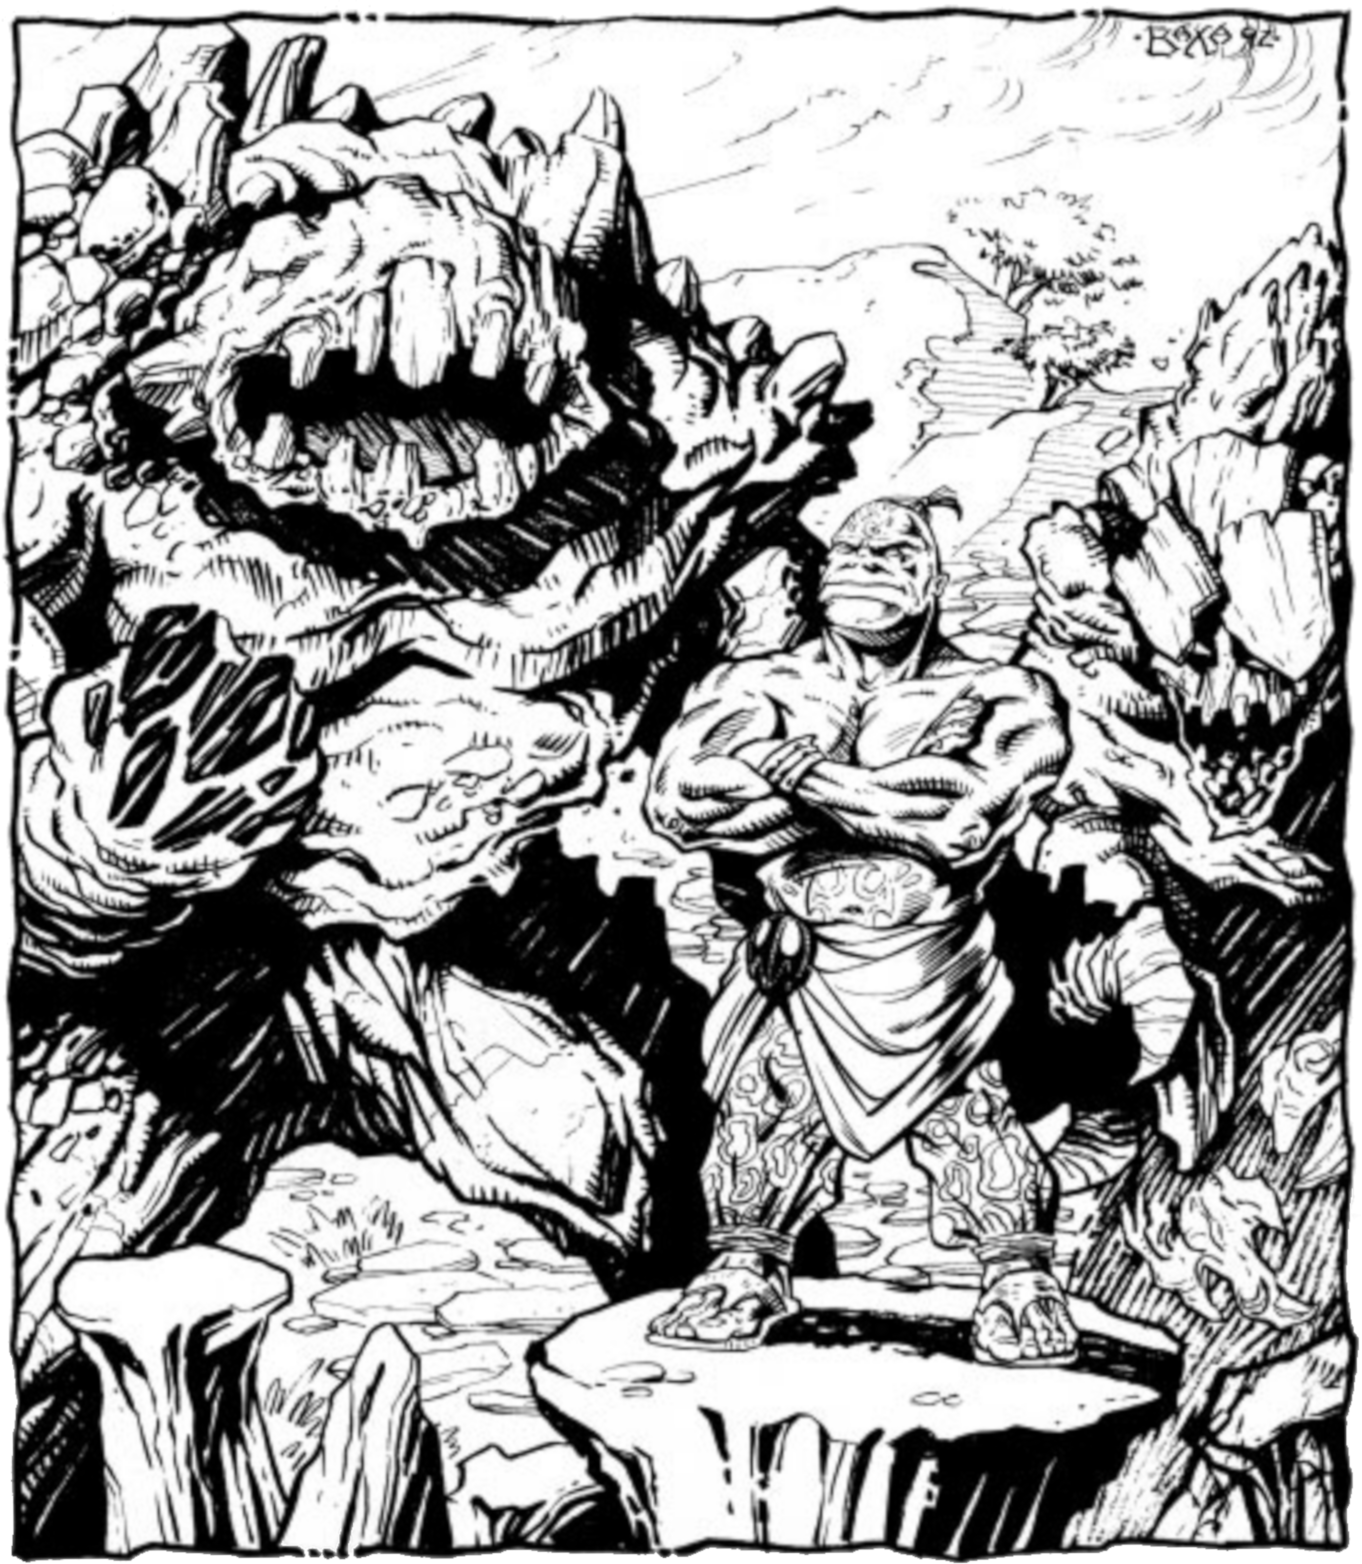
\includegraphics[width=\textwidth-2cm]{images/cleric-5.png}
% \WOTC
% \end{figure*}
\section{Divine Spells}
Clerics, druids, experienced rangers, and templars can cast divine spells. Unlike arcane spells, divine spells draw power from a divine source. Clerics forge a pact with a particular element, and draw their power from the elemental planes themselves. Rangers learn to manipulate minor nature spirits, druids are granted their powers directly from the spirits of the lands, while templars are gifted with spell by their sorcerer-kings.

\subsection{Preparing Divine Spells}
Divine spellcasters prepare their spells in largely the same manner as wizards do, but with a few differences. The relevant ability for divine spells is Wisdom. To prepare a divine spell, a character must have a Wisdom score of 10 + the spell's level. Likewise, bonus spells are based on Wisdom.

\Figure*{b}{images/cleric-6.png}

\textbf{Time of Day:} A divine spellcaster chooses and prepares spells ahead of time, just as a wizard does. However, a divine spellcaster does not require a period of rest to prepare spells. Instead, the character chooses a particular part of the day to pray and receive spells. The time is usually associated with some daily event. If some event prevents a character from praying at the proper time, he must do so as soon as possible. If the character does not stop to pray for spells at the first opportunity, he must wait until the next day to prepare spells.

\textbf{Spell Selection and Preparation:} A divine spellcaster selects and prepares spells ahead of time through prayer and meditation at a particular time of day. The time required to prepare spells is the same as it is for a wizard (1 hour), as is the requirement for a relatively peaceful environment. A divine spellcaster does not have to prepare all his spells at once. However, the character's mind is considered fresh only during his or her first daily spell preparation, so a divine spellcaster cannot fill a slot that is empty because he or she has cast a spell or abandoned a previously prepared spell.

Divine spellcasters do not require spellbooks. However, such a character's spell selection is limited to the spells on the list for his or her class. Clerics, druids, rangers, and templars have separate spell lists. A cleric also has access to two domains determined during his character creation. Each domain gives him access to a domain spell at each spell level from 1st to 9th, as well as a special granted power. With access to two domain spells at each spell level---one from each of his two domains---a cleric must prepare, as an extra domain spell, one or the other each day for each level of spell he can cast. If a domain spell is not on the cleric spell list, it can be prepared only in a domain spell slot.

\textbf{Spell Slots:} The character class tables show how many spells of each level a character can cast per day.

These openings for daily spells are called spell slots. A spellcaster always has the option to fill a higher-level spell slot with a lower level spell. A spellcaster who lacks a high enough ability score to cast spells that would otherwise be his or her due still gets the slots but must fill them with spells of lower level.

\textbf{Recent Casting Limit:} As with arcane spells, at the time of preparation any spells cast within the previous 8 hours count against the number of spells that can be prepared.

\textbf{Spontaneous Casting of Cure and Inflict Spells:} A good cleric (or a cleric of a good deity) can spontaneously cast a \spellref{cure light wounds}{cure} spell in place of a prepared spell of the same level or higher, but not in place of a domain spell. An evil cleric (or a cleric of an evil deity) can spontaneously cast an \spellref{inflict light wounds}{inflict} spell in place of a prepared spell (one that is not a domain spell) of the same level or higher. Each neutral cleric of a neutral deity either spontaneously casts \spellref{cure light wounds}{cure} spells like a good cleric or \spellref{inflict light wounds}{inflict} spells like an evil one, depending on which option the player chooses when creating the character. The divine energy of the spell that the \spellref{cure light wounds}{cure} or \spellref{inflict light wounds}{inflict} spell substitutes for is converted into the cure or \spellref{inflict light wounds}{inflict} spell as if that spell had been prepared all along.

\textbf{Spontaneous Casting of Summon Nature's Ally Spells:} A druid can spontaneously cast a summon nature's ally spell in place of a prepared spell of the same level or higher. The divine energy of the spell that the summon nature's ally spell substitutes for is converted into the summon spell as if that spell had been prepared all along.

\subsubsection{Combined Casting}
Clerics of 7th level or higher can join forces to cast a spell from a paralemental domain. This special casting cannot be done by paraelemental clerics.

In order to cast this spell, the clerics must meet the conditions for casting:
\begin{itemize*}
\item The clerics must be in contact with the paraelements, or with each of their own elements.
\item The clerics must be in physical contact with each other, by joining hands for example.
\item Both clerics must perform whatever somatic, verbal, or material components necessary for the spell.
% \item The spell's casting time is doubled (see \tabref{Combine Casting}).
\item Both clerics use the domain slot of that spell level.
\end{itemize*}

The clerics make a combined casting by one of them choosing the delay action. In doing so, the one with higher initiative elects to act at the other cleric's initiative. Until the spell is cast, the one who delayed action takes no other action during that round. Casting a spell this way takes double the time a normal spell would take (see \tabref{Combined Casting}).

\Table{Combined Casting}{XX}{
  \tableheader Original Casting Time
& \tableheader New Casting Time \\
1 swift action         & 1 move action   \\
1 standard action      & 1 full round    \\
1 full round or longer & Double the time \\
}

If the clerics are of the same level but have different Wisdom modifiers, the spell DC is based on the lower modifier. If the clerics have different levels, the effects of the spell are based on the lower level cleric, such as the spell's range, damage, number of targets and the spell's DC. For all purposes, both clerics are treated as the caster, e.g. personal range spells, or \spell{spell turning} effects.

For example, Herak is a 9th-level fire cleric and Tella is a 7th-level earth priest. They want to combine powers and cast a spell of the Paraelemental Plane of Magma. Since they are standing in a rich field, Tella is in contact with her element, but there is no fire. Herak casts \spell{continual flame} to create magical fire to surround them. The first condition is met.

They decide to use the \spell{oil spray} spell. The clerics link hands, point their fingers at a small patch of earth and watch as a fountain of flammable oil spouts up. Since \spell{oil spray} is a 4th-level spell, both of them use their domain spell slot of 4th-level. They can still cast more combined spells depending on the domain spell slots available for both of them.


\BigTableBottom{Divine Patrons and Supplemental Domains}{lllcXl}{
  \tableheader Name
& \tableheader Type
& \tableheader Class
& \tableheader Alignment
& \tableheader Domains
& \tableheader Favored Weapon \\

Air
& Element
& Cleric
& ---
&
    Air,
    Forecasting,
    Freedom,
    Liberation\textsuperscript{CD},
    Pact\textsuperscript{CD}
& Short bow \\

Earth
& Element
& Cleric
& ---
&
    Agriculture,
    Community\textsuperscript{CD},
    Cycle,
    Earth,
    Pact\textsuperscript{CD}
& Quarterstaff \\

Fire
& Element
& Cleric
& ---
&
    Cleansing,
    Competition\textsuperscript{CD},
    Fire,
    Pact\textsuperscript{CD},
    Wrath
& Longsword \\

Water
& Element
& Cleric
& ---
&
    Creation\textsuperscript{CD},
    Pact\textsuperscript{CD},
    Purity,
    Replenishment,
    Water
& Spear \\

Magma
& Paraelement
& Cleric
& ---
&
    Drought,
    Fate\textsuperscript{CW},
    Magma,
    Pact\textsuperscript{CD}
& Battleaxe \\

Rain
& Paraelement
& Cleric
& ---
&
    Growth,
    Pact\textsuperscript{CD},
    Rain,
    Weather\textsuperscript{CD}
& Spear \\

Silt
& Paraelement
& Cleric
& ---
&
    Pact\textsuperscript{CD},
    Pestilence\textsuperscript{CD},
    Silt,
    Thirst
& Scythe \\

Sun
& Paraelement
& Cleric
& ---
&
    Mirage,
    Pact\textsuperscript{CD},
    Purification\textsuperscript{CD},
    Sun
& Heavy mace \\

Abalach-Re
& Sorcerer-Monarch
& Templar
& CE
&
    Chaos,
    Charm,
    Domination\textsuperscript{CD}
    % Tyranny\textsuperscript{CW}
& Dagger \\

Andropinis
& Sorcerer-Monarch
& Templar
& LE
&
    Law,
    Nobility,
    Planning\textsuperscript{CW}
& Dagger \\

Borys
& Sorcerer-Monarch
& Templar
& LE
&
    Destruction,
    Inquisition\textsuperscript{CD},
    Protection
& Short sword \\

Daskinor
& Sorcerer-Monarch
& Templar
& CE
&
    Chaos,
    Domination\textsuperscript{CD},
    Madness
    % Tyranny\textsuperscript{CW}
& Dagger \\

Dregoth
& Sorcerer-Monarch
& Templar
& CE
&
    Death,
    Destruction,
    Tyranny\textsuperscript{CW}
& Longsword \\

Hamanu
& Sorcerer-Monarch
& Templar
& LE
&
    Courage\textsuperscript{CW},
    Strength,
    War
& Longsword \\


Kalak
& Sorcerer-Monarch
& Templar
& NE
&
    Magic,
    Mysticism\textsuperscript{CD},
    Trickery
& Dagger \\

Lalali-Puy
& Sorcerer-Monarch
& Templar
& LE
&
    Animal,
    Plant,
    Summoner\textsuperscript{CD}
& Spear \\

Nibenay
& Sorcerer-Monarch
& Templar
& LE
&
    Magic,
    Mind,
    Mysticism\textsuperscript{CD}
& Longsword \\

Oronis
& Sorcerer-Monarch
& Templar
& NG
&
    Knowledge,
    Planning\textsuperscript{CW},
    Protection
& Quarterstaff \\

Tectuktitlay
& Sorcerer-Monarch
& Templar
& NE
&
    Courage\textsuperscript{CW},
    Glory,
    Strength
& Dagger \\

\BigTableNote{6}{\textit{Special:} Air and rain wanderers may choose the Celerity\textsuperscript{CD} domain instead of the Travel domain.}\\
}


\subsection{Templars}
Templars cast divine spells, but they do not prepare their spells. A templar's class level limits the number of spells he can cast. %His high Charisma score might allow him to cast a few extra spells. A templar must have a Charisma score of at least 10 + a spell's level to cast the spell.

\textbf{Daily Readying of Spells:} Each day, templars must focus their minds on the task of casting their spells. A templar needs 8 hours of rest (just like a cleric), after which he spends 15 minutes concentrating. During this period, the templar readies his mind to cast his daily allotment of spells. Without such a period to refresh himself, the character does not regain the spell slots he used up the day before.

\textbf{Recent Casting Limit:} As with clerics, any spells cast within the last 8 hours count against the templar's daily limit.

\textbf{Adding Spells to a Templar's Repertoire:} A templar gains spells each time he attains a new level in his class and never gains spells any other way. Templars automatically know all spells on the templar's spell list, for each spell level they can cast. With permission, templars can also select the spells they gain from new and unusual spells that they have gained some understanding of.

\subsection{Divine Magical Writings}
Divine spells can be written down and deciphered just as arcane spells can (see Arcane Magical Writings). Any character with the \skill{Spellcraft} skill can attempt to decipher the divine magical writing and identify it. However, only characters who have the spell in question (in its divine form) on their class spell list can cast a divine spell from a scroll.

\subsection{New Divine Spells}
Divine spellcasters most frequently gain new spells in one of the following two ways.

\textbf{Spells Gained at a New Level:} Characters who can cast divine spells undertake a certain amount of study between adventures. Each time such a character receives a new level of divine spells, he or she learns new spells from that level automatically.

\textbf{Independent Research:} A divine spellcaster also can research a spell independently, much as an arcane spellcaster can. Only the creator of such a spell can prepare and cast it, unless he decides to share it with others.

\subsection{Domains From Other Sources}
The \emph{Complete Divine} and \emph{Complete Warrior} supplements introduce new domains. While not all domains from those supplements fit the {\tableheader Dark Sun} theme, \tabref{Divine Patrons and Supplemental Domains} shows all domains each divine patron provides.

\textbf{Domain Equivalencies:} In order to select domain feats\textsuperscript{CC}, a character must choose a domain within their patron's sphere of influence. The following table provides equivalencies for all domains granted by divine patrons of {\tableheader Dark Sun}. This list differs from the \emph{Complete Champion} supplement in some cases, so we advocate using this list as reference instead.

\Table{Supplemental Domain Equivalencies}{lXX}{
  \tableheader Class
& \tableheader Domain
& \tableheader Equivalent Domain Feat \\
Cleric & Agriculture   & Plant Devotion\textsuperscript{CC} \\
Cleric & Cleansing     & Strength Devotion\textsuperscript{CC} \\
Cleric & Cycle         & Death Devotion\textsuperscript{CC} \\
Cleric & Decay         & Destruction Devotion\textsuperscript{CC} \\
Cleric & Drought       & Death Devotion\textsuperscript{CC} \\
Cleric & Forecasting   & Air Devotion\textsuperscript{CC} \\
Cleric & Freedom       & Luck Devotion\textsuperscript{CC} \\
Cleric & Growth        & Animal Devotion\textsuperscript{CC} \\
Cleric & Magma         & Fire Devotion\textsuperscript{CC} \\
Cleric & Mirage        & Trickery Devotion\textsuperscript{CC} \\
Cleric & Purity        & Protection Devotion\textsuperscript{CC} \\
Cleric & Rain          & Water Devotion\textsuperscript{CC} \\
Cleric & Replenishment & Healing Devotion\textsuperscript{CC} \\
Cleric & Silt          & Earth Devotion\textsuperscript{CC} \\
Cleric & Wrath         & War Devotion\textsuperscript{CC} \\
Cleric & Community\textsuperscript{CD}    & Protection Devotion\textsuperscript{CC} \\
Cleric & Competition\textsuperscript{CD}  & War Devotion\textsuperscript{CC} \\
Cleric & Creation\textsuperscript{CD}     & Healing Devotion\textsuperscript{CC} \\
Cleric & Fate\textsuperscript{CW}         & Luck Devotion\textsuperscript{CC} \\
Cleric & Liberation\textsuperscript{CD}   & Good Devotion\textsuperscript{CC} \\
Cleric & Pact\textsuperscript{CD}         & Protection Devotion\textsuperscript{CC} \\
Cleric & Pestilence\textsuperscript{CD}   & Destruction Devotion\textsuperscript{CC} \\
Cleric & Purification\textsuperscript{CD} & Healing Devotion\textsuperscript{CC} \\
Cleric & Weather\textsuperscript{CD}      & Air Devotion\textsuperscript{CC} \\

Templar & Charm         & Trickery Devotion\textsuperscript{CC} \\
Templar & Glory         & Sun Devotion\textsuperscript{CC} \\
Templar & Madness       & Chaos Devotion\textsuperscript{CC} \\
Templar & Mind          & Knowledge Devotion\textsuperscript{CC} \\
Templar & Nobility      & Protection Devotion\textsuperscript{CC} \\
Templar & Courage\textsuperscript{CW}      & Strength Devotion\textsuperscript{CC} \\
Templar & Domination\textsuperscript{CD}   & Magic Devotion\textsuperscript{CC} \\
Templar & Inquisition\textsuperscript{CD}  & Law Devotion\textsuperscript{CC} \\
Templar & Mysticism\textsuperscript{CD}    & Magic Devotion\textsuperscript{CC} \\
Templar & Planning\textsuperscript{CW}     & Knowledge Devotion\textsuperscript{CC} \\
Templar & Summoner\textsuperscript{CD}     & Animal Devotion\textsuperscript{CC} \\
Templar & Tyranny\textsuperscript{CW}      & Evil Devotion\textsuperscript{CC} \\

Wanderer & Celerity\textsuperscript{CD}     & Travel Devotion\textsuperscript{CC} \\

}
